\documentclass[a4paper, 12pt]{article}
\usepackage{float}
\usepackage{listings}
\usepackage[total={18cm, 20cm}]{geometry}
\usepackage{graphicx}

\title{Writing a Loop-Sum Program for Jasmin Assembler}
\date{November 6, 2019}
\author{201704150 Kangjun Heo}

\lstset{basicstyle=\footnotesize\ttfamily,
        breaklines=true}

\begin{document}
    \maketitle

    \begin{abstract}
        Jasmin assembler is an assembler for Java Virtual Machine(JVM). I implemented a program for JVM that prints sum of 1 to 100, with the assembler and its language.
    \end{abstract}

    \tableofcontents

    \section{Introduction}
    Jasmin assembler is an assembler for Java Virtual Machine, provides several mnemonics for understandings of JVM bytecode.\cite{oracle_isa} It is not only enables human to write JVM program directly without any high-level languages, but also offers actual comprehensions of the program(being called \textit{Summer} from now). For this assignment, I wrote a designated program which gets no input but prints sum of 1 to 100.

    \section{Implementation}
    The entry point \textit{Summer} is \texttt{Sum.main(String[])}, which calls \texttt{Sum.sum(int)} returns \texttt{int}.

        \subsection{Class Definition}
        Every java program has classes, so I declared a class that named \texttt{Sum} for \textit{Summer}.
        \begin{figure}[H]
            \begin{lstlisting}[gobble=8]
            .class public Sum
            .super java/lang/Object
            \end{lstlisting}
    
            \centering        
            \caption{Declaration of class \texttt{Sum}}
        \end{figure}
        Since every objects (except primitive data) in JVM is derived from \texttt{java.lang.Object}, So I put an explicit super class information.  

        \subsection{Methods}
        According to specification, it is required to get sum value from subroutine, thus method \texttt{sum} is declared.

        \begin{figure}[H]
            \begin{lstlisting}[gobble=8]
            public static int  sum(int max)
            public static void main(String[] args)
            \end{lstlisting}
    
            \centering        
            \caption{Methods intended to implement}
        \end{figure}

        These methods can be written in this form:

        \begin{figure}[H]
            \begin{lstlisting}[gobble=8]
            .method public static sum(I)I
            .method public static main([Ljava/lang/String;)V
            \end{lstlisting}
    
            \centering        
            \caption{Methods actually implemented}
        \end{figure}

        \subsection{Loop Implementation}
        Loop should be continued until iteration variable reaches \texttt{max}, the integer typed argument od the method. This pseudocode snippet describes the total workflow of method \texttt{sum(int)}:
        \begin{figure}[H]
            \begin{lstlisting}[gobble=8]
            int sum = 0;

            for (int i = 1; i <= max; ++i) 
                sum += i;

            return sum;
            \end{lstlisting}
    
            \centering        
            \caption{Pseudocode in Java}
        \end{figure}

        Thus, the actual jasmin code is written in this form:

        \begin{figure}[H]
            \begin{lstlisting}[gobble=8]
            ; inside of sum(I)I
                ldc 0
                istore 1
            
                ldc 1
                istore 2
            
            Sum_Loop:
                iload 1     
                iload 2
                iadd
                istore 1      ; sum = sum + i
                
                iload 2
                iload 0
                isub          ; check = i - sum
            
                iinc 2 1
                ifne Sum_Loop ; return to Sum_Loop when check is not 0
            
                iload 1
                ireturn       ; return sum
            \end{lstlisting}
    
            \centering        
            \caption{Actual loop implementation for result of sum}
        \end{figure}
        
        \subsection{Errors}
        I suffered with several unknown errors which prevents successful testing during the implementation, for example, \texttt{java.lang.ClassFormatError} and \texttt{java.lang.VerifyError}. I had to fix it without any assistance of debugger or analyzer, thus I need to google and ask some help to Prof. Cho. 
    
            \subsubsection{\texttt{ClassFormatError}}
            \texttt{ClassFormatError} is an error that is thrown when the Java Virtual Machine attempts to read a class file and determines that the file is malformed or otherwise cannot be interpreted as a class file. \cite{oracle_cfe} It is the issue that I encountered for the first time, Actual output of error message was:
            
            \begin{figure}[H]
                \begin{lstlisting}[gobble=20]
                    Error: A JNI error has occurred, please check your installation and try again
                    Exception in thread "main" java.lang.ClassFormatError: Field "out" in class Sum has illegal signature "Ljava/io/PrintStream"
                            at java.lang.ClassLoader.defineClass1(Native Method)
                            at java.lang.ClassLoader.defineClass(Unknown Source)
                            at java.security.SecureClassLoader.defineClass(Unknown Source)
                            at java.net.URLClassLoader.defineClass(Unknown Source)
                            at java.net.URLClassLoader.access$100(Unknown Source)
                            at java.net.URLClassLoader$1.run(Unknown Source)
                            at java.net.URLClassLoader$1.run(Unknown Source)
                            at java.security.AccessController.doPrivileged(Native Method)
                            at java.net.URLClassLoader.findClass(Unknown Source)
                            at java.lang.ClassLoader.loadClass(Unknown Source)
                            at sun.misc.Launcher$AppClassLoader.loadClass(Unknown Source)
                            at java.lang.ClassLoader.loadClass(Unknown Source)
                            at sun.launcher.LauncherHelper.checkAndLoadMain(Unknown Source)
                \end{lstlisting}
        
                \centering        
                \caption{Error message on first test execution}
            \end{figure}

            I checked the body of method \texttt{main} and figured out that semicolon is omitted in \texttt{getstatic} instruction, after \texttt{PrintStream}.
    
            \subsubsection{\texttt{VerifyError}}
            \texttt{VerifyError} is an another error I encountered, after resolving \texttt{ClassFormatError}. This error is thrown when the "verifier" detects that a class file, though well formed, contains some sort of internal inconsistency or security problem. \cite{oracle_ve}
    
            \begin{figure}[H]
                \begin{lstlisting}[gobble=20]
                    Error: A JNI error has occurred, please check your installation and try again
                    Exception in thread "main" java.lang.VerifyError: (class: Sum, method: sum signature: (I)I) Illegal local variable number
                            at java.lang.Class.getDeclaredMethods0(Native Method)
                            at java.lang.Class.privateGetDeclaredMethods(Unknown Source)
                            at java.lang.Class.privateGetMethodRecursive(Unknown Source)
                            at java.lang.Class.getMethod0(Unknown Source)
                            at java.lang.Class.getMethod(Unknown Source)
                            at sun.launcher.LauncherHelper.validateMainClass(Unknown Source)
                            at sun.launcher.LauncherHelper.checkAndLoadMain(Unknown Source)
                \end{lstlisting}
        
                \centering        
                \caption{Error message after \texttt{ClassFormatError} is resolved}
            \end{figure}

            According to Prof. Cho's Advice, each methods that have local variable or function calls in their body must limit the count of stack and local entries. I didn't give such directives to method \texttt{sum(I)I}, and after fix it, the error no longer occured, executed successfully.
    \section{Testing}
    \begin{figure}[H]
        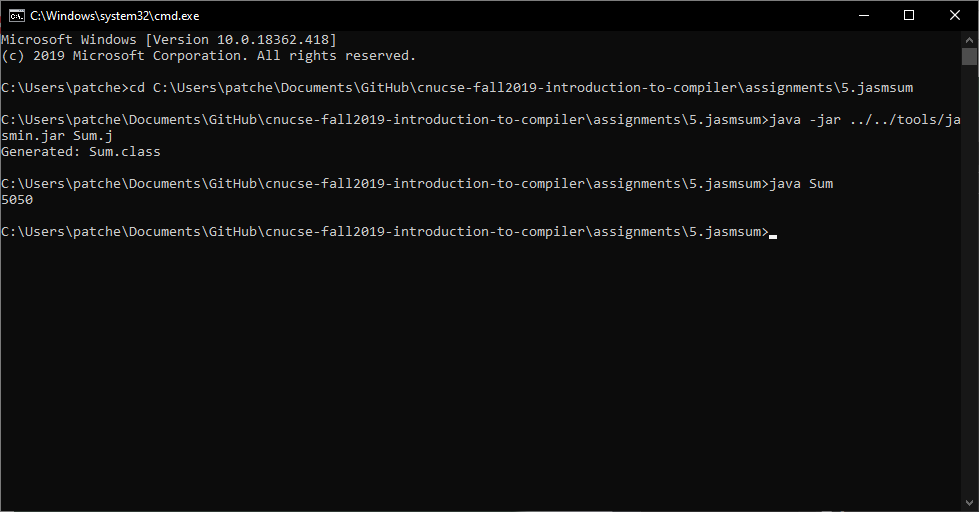
\includegraphics[width=\textwidth]{proof}

        \centering        
        \caption{Actual Testing Result}
    \end{figure}


    \section{Conclusion}
    In machine level, there are no \texttt{for} or \texttt{while} keywords exist in instruction set architecture, but conditional jumping instruction does the role instead. Also, if there are any local variable or function call, \texttt{.limit} directives are required to create enough space for such data.

    \section{Entire Source Code}

    \begin{lstlisting}[gobble=8]
        ; Sum.j
        ;
        ; Introduction to Compiler
        ; Assignment 5-1
        ; ------------------------
        ; 201704150 Kangjun Heo
        ; 
        ; This Java Assembly is written in manual, for Jasmin Assembler.
        ; The program calls a function sum(int) and prints its return value.
        
        .class public Sum
        .super java/lang/Object
        
        ; 
        ; class object initializer 
        ;
        .method public <init>()V
            aload_0
            invokespecial java/lang/Object/<init>()V
            return
        .end method
        
        ;
        ; method sum(int)
        ;
        ; returns int
        ; paramter n : int
        ;
        ; this method takes a integer typed value, 
        ; returns a integer typed sum of 1 to n.
        ;
        .method public static sum(I)I
            .limit stack 8
            .limit locals 16
        
            ; int sum = 0
            ldc 0
            istore 1
        
            ; int i = 1
            ldc 1
            istore 2
        
            ; Loop start 
        Sum_Loop:
            ; sum = sum + i;    
            iload 1
            iload 2
            iadd
            istore 1
            
            ; i - arg0
            iload 2
            iload 0
            isub
        
            ; ++i
            iinc 2 1
        
            ; test i == arg0 (from ln 51~53, check if not zero)
            ifne Sum_Loop
        
            ; Return 
            iload 1
            ireturn
        .end method
        
        ;
        ; method main(String[])
        ;
        ; returns nothing 
        ; parameter args : String[]
        ;
        ; this method is an entry point of Sum Java Program.
        ;
        .method public static main([Ljava/lang/String;)V
            ; limit maximum count of stack items and local variables
            .limit stack 8
            .limit locals 16
        
            ; get System.out static PrintStream object
            getstatic java/lang/System/out Ljava/io/PrintStream;
        
            ; call sum(100)
            ldc 100
            invokestatic Sum/sum(I)I
        
            ; call System.out.println(/* return value of sum(100) */)
            invokevirtual java/io/PrintStream/println(I)V
        
            return
        .end method
    \end{lstlisting}

    \bibliographystyle{plain}
    \bibliography{oracle_isa, oracle_cfe, oracle_ve}
\end{document}